\documentclass[a4paper,hidelinks,14pt]{extarticle}

\usepackage[utf8]{inputenc}
\usepackage[T2A]{fontenc}
\usepackage[english, russian]{babel}
\usepackage{lipsum}
\usepackage{amsmath}
\usepackage{amssymb}
\usepackage{amsfonts}
\usepackage{mathtools}
\usepackage{datetime}
\usepackage[pdftex]{graphicx}
\usepackage{indentfirst}
\usepackage{asymptote}
\usepackage{systeme}
\usepackage[dvipsnames]{xcolor}
\usepackage{lastpage}
\usepackage{fancybox,fancyhdr}
\usepackage{hyperref}
\usepackage[font={small,it}]{caption}
\fancyhead[L]{Курсовая работа}
\fancyhead[C]{}
\fancyhead[R]{\textit{Адаптивная компенсация возмущения}}
\fancyfoot[L]{}
\fancyfoot[C]{\thepage\space}
\fancyfoot[R]{}
\pagestyle{fancy}
\newcommand{\gt}{\textgreater}
\newcommand{\lt}{\textless}
\usepackage{listings}
\usepackage{xcolor}
\lstset{
    basicstyle=\ttfamily\small,
    keywordstyle=\color{blue},
    commentstyle=\color{gray},
    stringstyle=\color{red},
    numbers=left,
    numberstyle=\color[gray]{0.7}\ttfamily\small,
    stepnumber=1,
    numbersep=8pt,
    frame=single,
    showstringspaces=false,
    tabsize=4,
    breaklines=true
}
\usepackage{subcaption}

\begin{document}
	\begin{titlepage}
		\setlength{\parindent}{0ex}
		
		\begin{center}
			\textsc{
				\vspace{1ex}
                Научно-исследовательский университет ИТМО \\
				\vspace{0.5ex}
				Факультет систем управления и робототехники \\
				\vspace{0.5ex}
			}
		\end{center}
		
		\vspace{40mm}
		
		\begin{center}
			Курсовой проект по адаптивному управлению \\[0.5ex]
			\textbf{Адаптивная ускоренная компенсация \\
			мультисинусоидальных возмущений} \\[0.5ex]
			Вариант 7
		\end{center}

		% Схема Лайона
		
		\vspace{46mm}
		
		\begin{minipage}{.45\linewidth}
			Выполнил студент
            \\
			Преподаватель
		\end{minipage}
		\hfill
		\begin{minipage}{.52\linewidth}
			\begin{flushright}
				Мовчан Игорь Евгеньевич, R3480
				\\
				Парамонов Алексей Владимирович
			\end{flushright}
		\end{minipage}
		
		\vfill
		\begin{center}
			Санкт-Петербург
			\\
			2026
		\end{center}
		
	\end{titlepage}

	\tableofcontents
	\clearpage
	
	\section{Цель работы}
	Освоение принципа адаптивной ускоренной компенсации мультисинусоидальных возмущения на примере задачи стабилизации многомерного линейного объекта.
	
	\section{Постановка задачи}
	Рассмотрим задачу компенсации внешнего возмущения, действующего на объект с начальными условиями $x(0)$
	\begin{equation}
		\begin{cases}
			\dot{x} = Ax + bu + df \\
			y = Cx
		\end{cases}	
	\end{equation}

	Здесь $x \in \mathbb{R}^n$ - \textit{измеряемый} вектор состояния, $u$, $y$ - \textit{измеряемые} вход и выход объекта (скаляры), $A$, $b$, $C$ и $d$ - \textit{известные} матрицы соответствующих размерностей, $f$ - \textit{неизмеряемое} мультисинусоидальное возмущение с \textit{априори неизвестными} амплитудами, частотами и фазами гармоник.
	
	Также примем допущение, что сигналы $u$ и $f$ согласованы, а вектора $b$ и $d$ для простоты и наглядности равны.

	Цель задачи заключается в построении адаптивного управления, компенсирующего неизвестное возмущение так, чтобы
	\begin{equation}
		\lim_{t \to \infty} \|x(t)\| = 0. \label{3}
	\end{equation}

	Кроме того, необходимо применить специальную схему Лайона, обеспечивающую ускоренную параметрическую сходимость.

	\section{Управляемость и наблюдаемость}
	Для начала зададимся матрицей $A$ системы, вектором управления $b$, вектором наблюдения $C$, а также мультисинусоидальным воздействием $f$ согласно взятому варианту:
	\[
		A = \begin{bmatrix}
			0 & 1 \\
			9 & 2
		\end{bmatrix}, \quad
		b = d = \begin{bmatrix}
			9 \\
			5
		\end{bmatrix}, \quad
		C = \begin{bmatrix}
			3 & 3
		\end{bmatrix}
	\]
	\[
		f(t) = \cos(t + 9)\sin(8t-7) = \frac{\sin(9t + 2)}{2} + \frac{\sin(7t - 16)}{2}
	\]

	Любое построение управления для какой-либо системы стоит начать с проверки её управляемости и наблюдаемости. Сделаем это, вычислив матрицы управляемости $U$ и наблюдаемости $W$, проверив полноту их ранга:
	\[
		U = \begin{bmatrix}
			b & Ab
		\end{bmatrix} = \begin{bmatrix}
			9 & 5 \\
			5 & 91
		\end{bmatrix}, \quad W = \begin{bmatrix}
			C \\
			CA
		\end{bmatrix} = \begin{bmatrix}
			3 & 3 \\
			27 & 9
		\end{bmatrix}
	\]
	\[
		\text{rank}(U) = \text{rank}(W) = 2
	\]

	Их ранги полные, значит, система является полностью управляемой и наблюдаемой. Теперь можем перейти к синтезу управления.

	\section{Синтез адаптивного управления}
	Цель управления, как указано в \eqref{3}, заключается в асимптотической стабилизации состояния объекта $x(t)$ в условиях параметрически неопределенного возмущения $f(t)$. Для достижения этой цели синтезируем закон управления в виде суммы двух компонент:
	\begin{equation}
	u(t) = u_{\text{с}}(t) + u_{\text{к}}(t)
	\end{equation}

	Здесь $u_{\text{с}}(t)$ — стабилизирующее управление, а $u_{\text{к}}(t)$ — адаптивная компонента, предназначенная для компенсации возмущения.

	\subsection{Стабилизирующее управление}
	В качестве стабилизирующего управления веберем линейный регулятор обратной связью $K$:
	\begin{equation}
	u_{\text{с}}(t) = -K x(t)
	\end{equation}

	Подстановка этого управления в исходную систему дает:
	\[
	\dot{x} = (A - b K)x + b(u_{\text{к}} + f)
	\]

	Обратную связь $K$ необходимо выбрать так, чтобы матрица замкнутой системы $A_M = A - b K$ была гурвицевой. Для этого используем LQR-регулятор, минимизирующий функционал качества
	\[
		J = \int_0^\infty x^T(\tau) Q x(\tau) + r u^2(\tau) d\tau
	\]

	Расчет будем производить на основе уравнения Риккати относительно положительно определенной матрицы $P \succ 0$ с взятыми матрицей $Q = I \succcurlyeq 0$ и параметром $r = 3 > 0$:
	\[
		A^T P + PA + Q - P b r^{-1} b^T P = 0
	\]

	Откуда
	\[
		P = \begin{bmatrix}
			0.2866 & 0.1493  \\
			0.1493 & 0.2618 
		\end{bmatrix} \succ 0
	\]

	Тогда матрицу $K$ обратной связи вычислим как
	\[
		K = r^{-1} b^T P = \begin{bmatrix}
			1.1087 & 0.8843
		\end{bmatrix}
	\]

	\subsection{Компенсирующее управление}
	Адаптивная компонента управления $u_{\text{к}}$ предназначена для компенсации возмущения $f$. Логично выбрать ее в виде оценки возмущения, взятой с обратным знаком:
	\begin{equation}
	u_{\text{к}}(t) = -\hat{f}(t)
	\end{equation}

	С учетом этого, уравнение системы принимает вид:
	\[
	\dot{x} = A_M x + b(f - \hat{f})
	\]

	Из уравнения видно, что если оценка $\hat{f}$ будет сходиться к истинному значению $f$, то ошибка компенсации $(f - \hat{f})$ будет стремиться к нулю, и, поскольку матрица $A_M$ устойчива, состояние $x(t)$ также будет стремиться к нулю.

	Для построения оценки $\hat{f}$ параметризуем возмущение
	\begin{equation}
	f = \theta_f^T\xi_f
	\end{equation}

	При принятых
	\[
		\theta_f^T = \begin{bmatrix}
			k_{f0} - l_0 & k_{f1} - l_1 & \dots k_{f(r-1)} - l_{r-1}
		\end{bmatrix}
	\]
	\[
		\xi_f^T = \left[ \frac{1}{K_f(s)}[f], \frac{s}{K_f(s)}[f], \dots, \frac{s^{n-1}}{K_f(s)}[f] \right]
	\]

	Вектор $\xi_f$ также является вектором состояния фильтра
	\begin{equation}
		\dot{\xi}_f = A_{0f} \xi_f + b_{0f} f	
	\end{equation}
	
	Здесь матрицы
	\[
		A_{0f} = \begin{bmatrix} 
			0 & 1 & \dots & 0 \\ 
			0 & 0 & \dots & 0 \\ 
			\vdots & \vdots & \ddots & 1 \\ 
			-k_{f0} & -k_{f1} & \dots & -k_{fr-1} 
			\end{bmatrix}, \quad 
			b_{0f} = \begin{bmatrix} 
			0 \\ \vdots \\ 0 \\ 1 
			\end{bmatrix}
	\]

	Мы выберем их с расчётом на оценку двух гармонических сигналов и фильтр $K(f)$, имеющего корнями $\lambda = 3$:
	\[
		K(f) = (s+3)^4 = s^4 + 12 s^3 + 54s^2 +108s + 81
	\]
	\[
	A_{0f} = \begin{bmatrix}
			0 & 1 & 0 & 0 \\
			0 & 0 & 1 & 0 \\
			0 & 0 & 0 & 1 \\
			-81 & -108 & -54 & -12
		\end{bmatrix}, \quad b_{0f} = \begin{bmatrix}
			0 \\
			0 \\
			0 \\
			1
		\end{bmatrix}
	\]
	
	Так как вход фильтра $f$ неизмеряемый, то вектор состояния $\xi_f$ не доступен прямому измерению, в связи с чем возникает необходимость в его оценке. Предлагается структура наблюдателя $\xi_f$:
	\begin{equation}
		\begin{cases*}
			\hat{\xi}_f = \eta + Nx \\
			\dot{\eta} = A_{0f} \eta + (A_{0f} N - NA)x - Nbu	
		\end{cases*}
	\end{equation}
	
	Тут матрица $N$ находится из равенства
	\[
		Nd = b_{0f} \quad \Rightarrow \quad N = \frac{1}{9}\begin{bmatrix}
			0 & 0 \\
			0 & 0 \\
			0 & 0 \\
			1 & 0
		\end{bmatrix}
	\]

	Собирая всё воедино, получаем первичную оценку выходной переменной генератора внешнего возмущения
	\begin{equation}
		\hat{f} = \theta^T_f \hat{\xi}_f
	\end{equation}

	\section{Градиентный алгоритм адаптации}
	Так как в $\theta_f^T$ остаются неизвестными параметры $l_i$, ставится дополнительная задача его оценки при помощи алгоритма адаптации
	\begin{equation}
		\dot{\hat{\theta}} = \gamma \hat{\xi}_f b^T P x
	\end{equation}

	При принятой $P$ - симметричной положительно определенной матрице, являющейся решением уравнения Ляпунова
	\[
		A_M^T P + P A_M = -Q, \quad Q = I \succ 0
	\]

	Откуда
	\[
		P = \begin{bmatrix}
			0.0552  &  0.0148 \\
			0.0148  &  0.1641
		\end{bmatrix} \succ 0
	\]

	Оценка внешнего возмущения тогда имеет вид
	\[
		\hat{f} = \hat{\theta}_f^T \hat{\xi}_f \quad \Rightarrow \quad u_\text{к} = -\hat{f} = - \hat{\theta}_f^T \hat{\xi}_f
	\]

	А значит, финальное управление
	\begin{equation}
		u = u_{\text{с}} + u_{\text{к}} = -K x - \hat{\theta}_f^T \hat{\xi}_f
	\end{equation}
	
	Промоделируем систему по схеме из рисунка \ref{fig:model} при нулевых начальных условиях и коэффициенте адаптации $\gamma = 7500$ - рисунки \ref{fig:u_aa}-\ref{fig:theta_aa} для расширенного времени и рисунки \ref{fig:u_aa_25}-\ref{fig:theta_aa_25} для времени моделирования $t = 25$.

	\begin{figure}
		\centering
		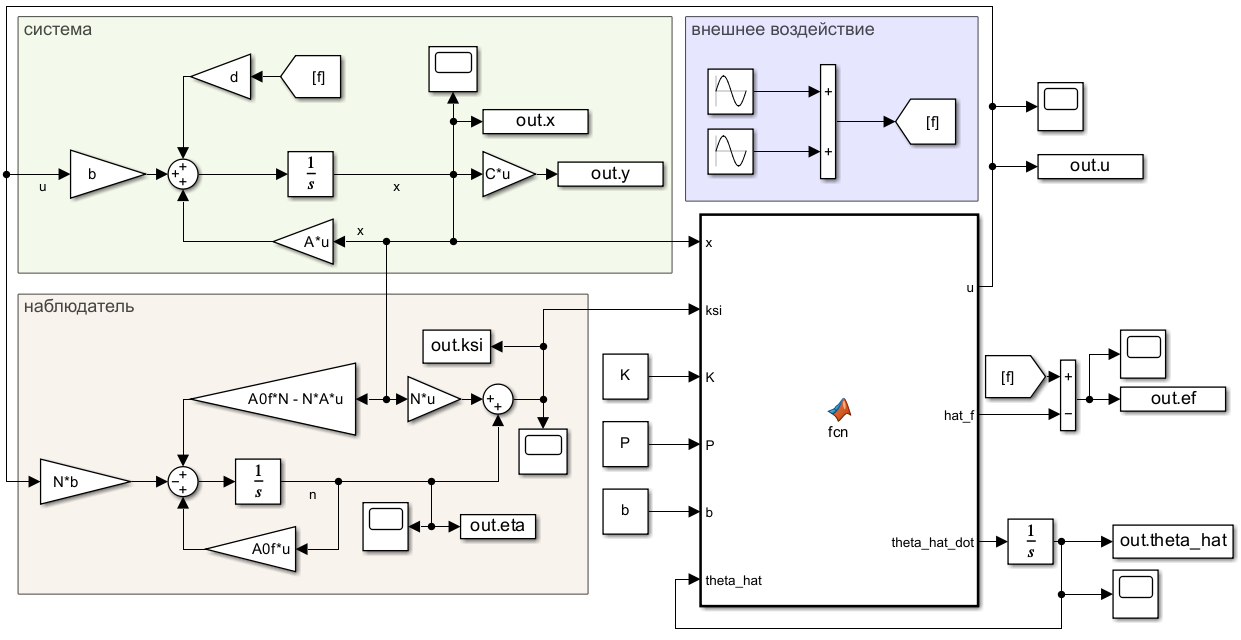
\includegraphics[width=\textwidth]{images/model.png}
		\caption{Модель системы с градиентным алгоритмом адаптации}
		\label{fig:model}
	\end{figure}
	\begin{figure}
		\centering
		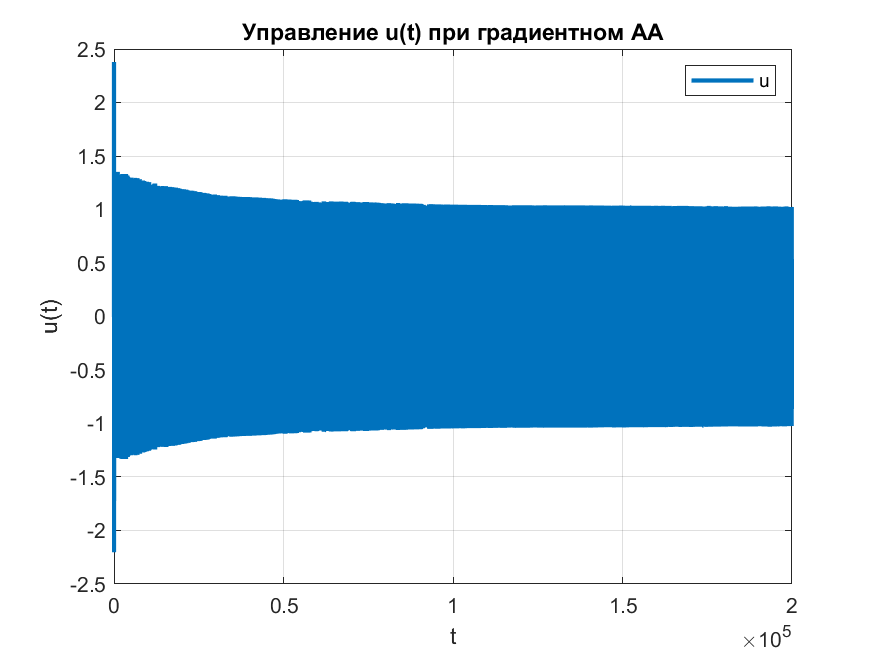
\includegraphics[width=0.8\textwidth]{images/u_aa.png}
		\caption{График управления при градиентном алгоритме адаптации}
		\label{fig:u_aa}
	\end{figure}
	\begin{figure}
		\centering
		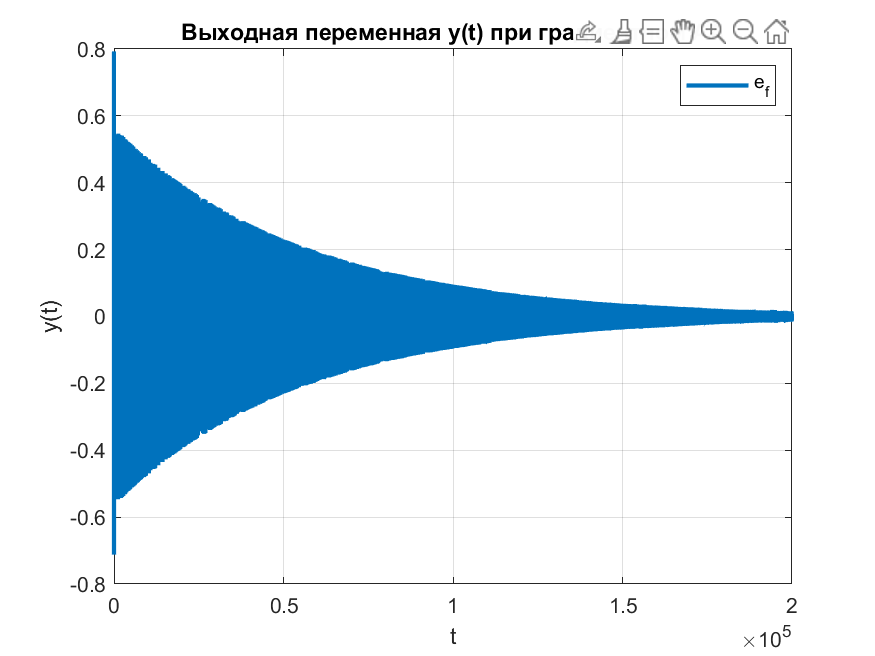
\includegraphics[width=0.8\textwidth]{images/y_aa.png}
		\caption{График выходной переменной при градиентном алгоритме адаптации}
		\label{fig:y_aa}
	\end{figure}
	\begin{figure}
		\centering
		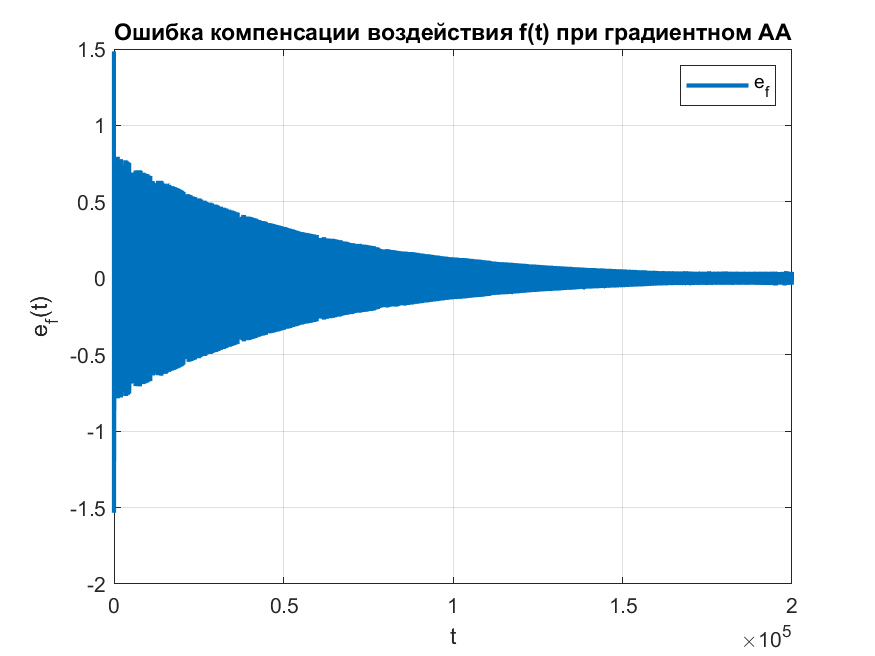
\includegraphics[width=0.8\textwidth]{images/ef_aa.png}
		\caption{График ошибки компенсации $f - \hat{f}$ при градиентном АА}
		\label{fig:ef_aa}
	\end{figure}
	\begin{figure}
		\centering
		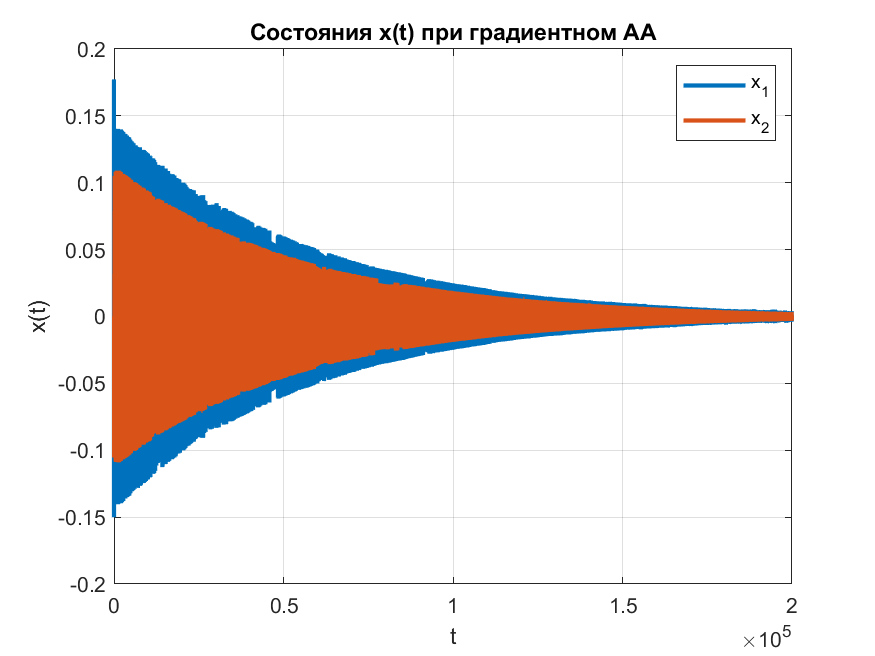
\includegraphics[width=0.8\textwidth]{images/x_aa.png}
		\caption{Графики состояний при градиентном алгоритме адаптации}
		\label{fig:x_aa}
	\end{figure}
	\begin{figure}
		\centering
		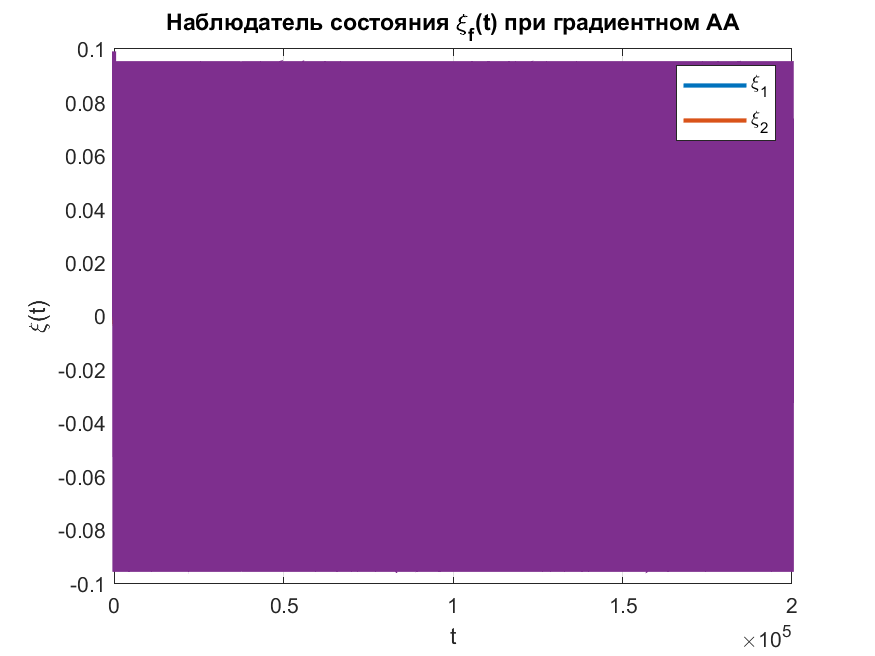
\includegraphics[width=0.8\textwidth]{images/xi_aa.png}
		\caption{График наблюдателей $\hat{\xi}_f(t)$ при градиентном алгоритме адаптации}
		\label{fig:xi_aa}
	\end{figure}
	\begin{figure}
		\centering
		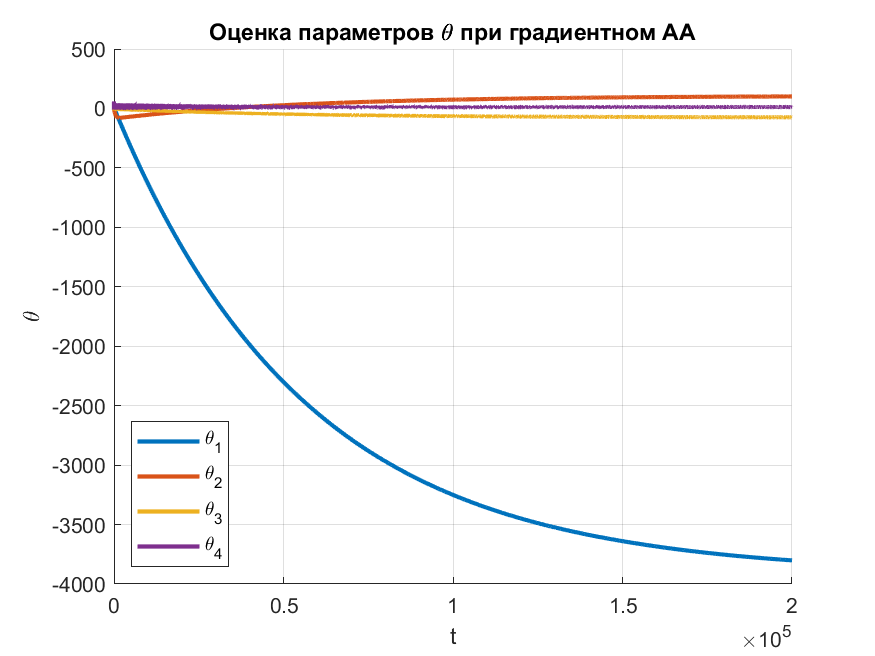
\includegraphics[width=0.8\textwidth]{images/theta_aa.png}
		\caption{График оценки $\theta$ при градиентном алгоритме адаптации}
		\label{fig:theta_aa}
	\end{figure}
	
	\begin{figure}
		\centering
		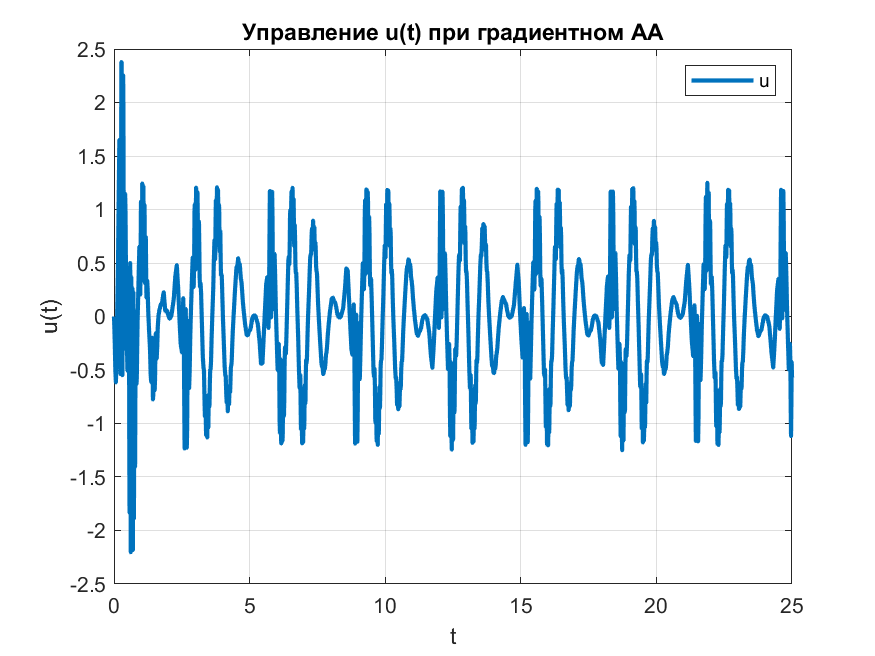
\includegraphics[width=0.8\textwidth]{images/u_aa_25.png}
		\caption{График управления при градиентном алгоритме адаптации и $t=25$}
		\label{fig:u_aa_25}
	\end{figure}
	\begin{figure}
		\centering
		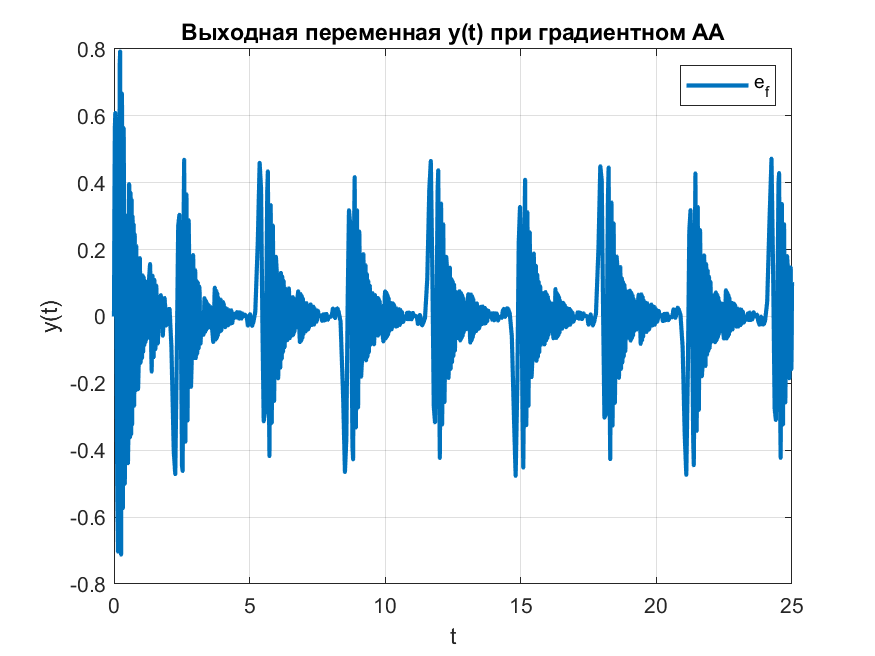
\includegraphics[width=0.8\textwidth]{images/y_aa_25.png}
		\caption{График выходной переменной при градиентном АА и $t=25$}
		\label{fig:y_aa_25}
	\end{figure}
	\begin{figure}
		\centering
		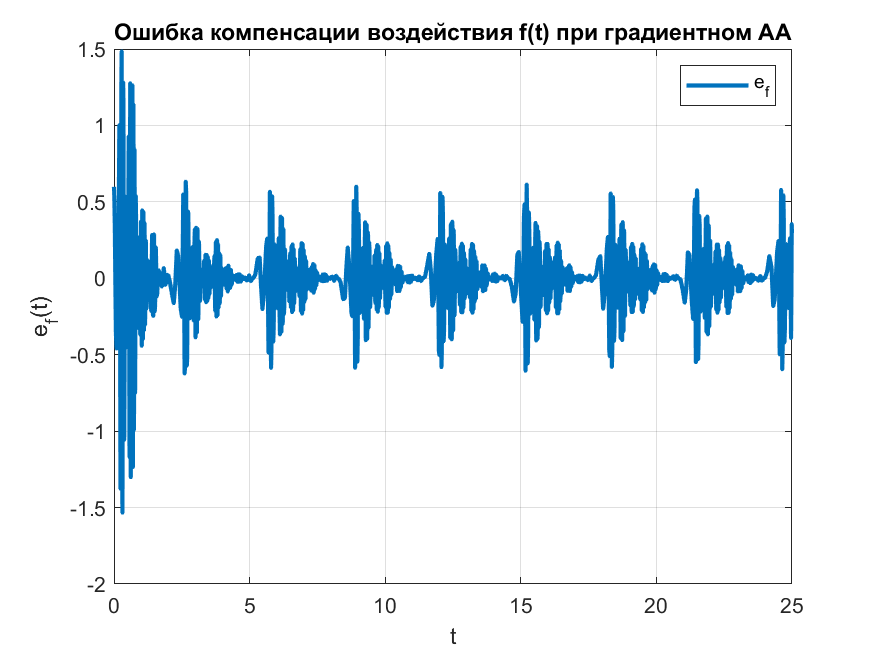
\includegraphics[width=0.8\textwidth]{images/ef_aa_25.png}
		\caption{График ошибки компенсации $f - \hat{f}$ при градиентном АА и $t=25$}
		\label{fig:ef_aa_25}
	\end{figure}
	\begin{figure}
		\centering
		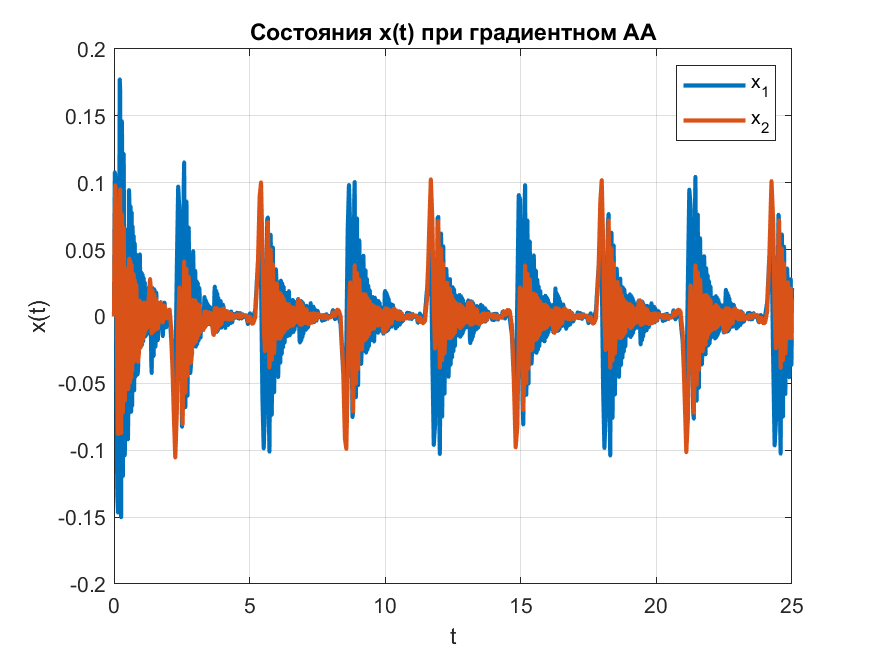
\includegraphics[width=0.8\textwidth]{images/x_aa_25.png}
		\caption{Графики состояний при градиентном алгоритме адаптации и $t = 25$}
		\label{fig:x_aa_25}
	\end{figure}
	\begin{figure}
		\centering
		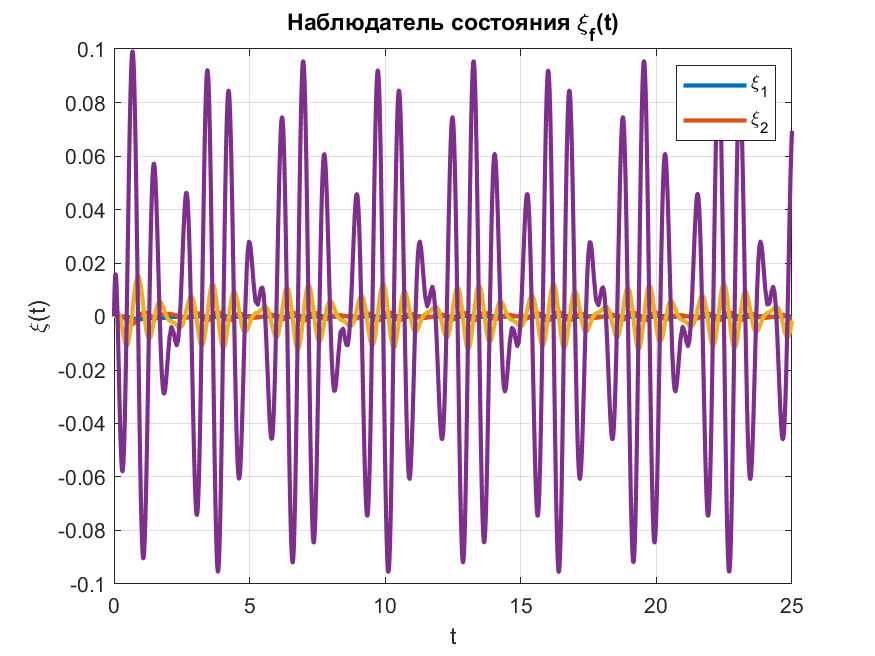
\includegraphics[width=0.8\textwidth]{images/xi_aa_25.png}
		\caption{График наблюдателей $\hat{\xi}_f(t)$ при градиентном АА и $t = 25$}
		\label{fig:xi_aa_25}
	\end{figure}
	\begin{figure}
		\centering
		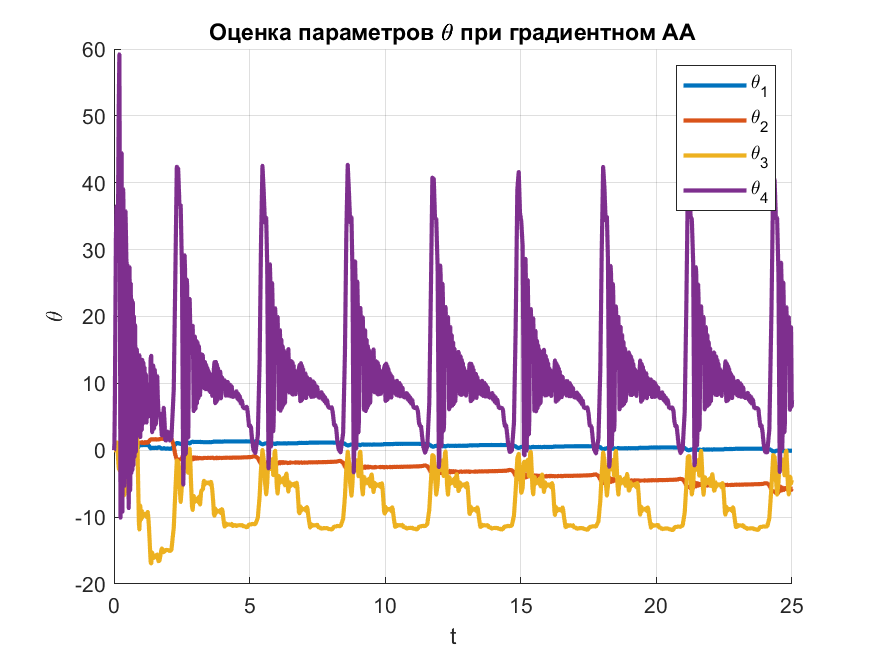
\includegraphics[width=0.8\textwidth]{images/theta_aa_25.png}
		\caption{График оценки $\theta$ при градиентном алгоритме адаптации и $t = 25$}
		\label{fig:theta_aa_25}
	\end{figure}

	На графиках можем видеть, что алгоритм компенсирует внешнее воздействие \textit{крайне} долго - лишь спустя $t = \cdot 2.5 \cdot 10^5$ секунд удалось добиться относительно низких значений состояний $x(t)$. При этом алгоритм не справляется с задачей идентификации параметров $\theta$. В связи с этим становится актуальной задача ускорения адаптации.

	\section{Ускоренная адаптация}
	Ускорение адаптации производится с помощью схемы Лайона, в которой используется модификация алгоритма настройки, основанная на динамическом расширении регрессора:
	\begin{equation}
		\dot{\hat{\theta}} = \gamma \Xi_f^T \left( \Xi_e + \Xi_{f\theta} - \Xi_{f\hat{\theta}} \right)
	\end{equation}
	
	Здесь $\Xi_f$, $\Xi_e$ и $\Xi_{f\theta}$ — сигналы, полученные путем специальной фильтрации переменных системы. 
	
	Для реализации ускоренной адаптации в качестве вектора регрессора используется оценка состояний генератора возмущения $\hat{\xi}_f$, полученная в предыдущем пункте. Вводится вспомогательный оператор $H(s)$, соответствующий передаточной функции замкнутой системы, и фильтры низких частот $L_i(s)$:
	\begin{equation}
		H(s) = b^T P (sI - A_M)^{-1} b, \quad L_i(s) = \frac{\lambda_i}{s + \lambda_i}, \quad i=1,\dots,q
	\end{equation}
	
	Согласно схеме метода, формируются группы сигналов:
	\begin{enumerate}
		\item \textbf{Фильтрованная матрица регрессора} $\Xi_f$. Каждый её элемент получается путем последовательного пропускания компонент вектора $\hat{\xi}_f$ через оператор $H(s)$ и фильтр $L_i(s)$:
		\begin{equation}
			(\Xi_f)_{ij} = L_i(s) \left[ H(s) [(\hat{\xi}_f)_j] \right]
		\end{equation}
		
		\item \textbf{Фильтрованная ошибка} $\Xi_e$. Скалярная ошибка стабилизации $e = b^T P x$ проходит только через фильтр $L_i(s)$:
		\begin{equation}
			(\Xi_e)_i = L_i(s) [e]
		\end{equation}
		
		\item \textbf{Сигнал компенсации} $\Xi_{f\theta}$. Воздействие $\hat{\theta}^T \hat{\xi}_f$ (при принятой $\hat{\theta}$ — текущая оценка) пропускается через цепочку фильтров:
		\begin{equation}
			(\Xi_{f\theta})_i = L_i(s) \left[ H(s) [\hat{\theta}^T \hat{\xi}_f] \right]
		\end{equation}
	\end{enumerate}

	Проведем моделирование системы с использованием модифицированного алгоритма при параметрах фильтров $\lambda = {5, 10, 15, 20}$ и коэффициенте адаптации $\gamma = 2000$. Результаты моделирования представлены на рисунках \ref{fig:u_lion}-\ref{fig:theta_lion}. 
	
	Видим, что качество процессов в сравнении с предыдущим методом улучшается в разы - сходимость быстрее, происходит идентификация $\theta$, а сами графики плавные!

	\begin{figure}
		\centering
		
\includegraphics[width=0.8\textwidth]{images/lyon_u.png}
		\caption{График управления при модифицированном алгоритме адаптации}
		\label{fig:u_lion}
	\end{figure}
	\begin{figure}
		\centering
		
\includegraphics[width=0.8\textwidth]{images/lyon_y.png}
		\caption{График выхода при модифицированном алгоритме адаптации}
		\label{fig:y_lion}
	\end{figure}
	\begin{figure}
		\centering
		
\includegraphics[width=0.8\textwidth]{images/lyon_ef.png}
		\caption{График ошибки компенсации $f - \hat{f}$ при модифицированном АА}
		\label{fig:ef_lion}
	\end{figure}
	\begin{figure}
		\centering
		
\includegraphics[width=0.8\textwidth]{images/lyon_x.png}
		\caption{Графики состояний при модифицированном алгоритме адаптации}
		\label{fig:x_lion}
	\end{figure}
	\begin{figure}
		\centering
		
\includegraphics[width=0.8\textwidth]{images/lyon_theta.png}
		\caption{График оценки $\theta$ при модифицированном алгоритме адаптации}
		\label{fig:theta_lion}
	\end{figure}

	\section{Общие выводы}
	В ходе лабораторной работы был освоен принцип адаптивной компенсации мультисинусоидальных возмущений на примере стабилизации многомерной линейной системы. Сравнительный анализ первичного метода и модифицированного показал, что использование схемы Лайона позволяет многократно повысить скорость сходимости и точность идентификации параметров по сравнению со стандартным градиентным алгоритмом.

	
\end{document}